% !Mode:: "TeX:UTF-8"
\chapter{系统实现}

这一部分主要阐述异构计算资源平台的具体实现过程,具体的实现细节。这一部分将以和系统设计相反的顺序,从底到上来阐述系统的实现,分别是系统环境配置,工具链构建,平台实现和接口实现。


\section{系统环境}

平台系统环境主要包括,实现平台的操作系统和硬件信息,平台依赖的底层软件安装和不同软件版本的管理方法。

\subsection{硬件环境}

本地的主机采用的是64位的Ubuntu系统,CPU为64位的intel i5 10210U,GPU为Nvidia MX250。内存为16G内存。

\subsection{软件环境}

平台需要依赖的软件众多,软件环境非常复杂,同时需要处理不同软件之间的版本依赖,平台所依赖的所有软件及其版本如下表\ref{platform_software}所示。

\begin{table}[h!]
    \centering
    \caption{软件环境}
    \label{platform_software}
    \begin{tabular}{c|c|c}
    \hline
                                 & 软件             & 版本          \\ \hline
    驱动                          & Nidia Driver   & 460.39      \\ \hline
    \multirow{3}{*}{GPU计算库}      & Cuda           & 11.1        \\ \cline{2-3} 
                                 & Cudnn          & 8.0.5       \\ \cline{2-3} 
                                 & OpenCL         & 2.2         \\ \hline
    \multirow{4}{*}{深度学习框架}      & Pytorch        & 1.8.1+cu111 \\ \cline{2-3} 
                                 & Tensorflow     & 2.4.1       \\ \cline{2-3} 
                                 & Keras          & 2.4.0       \\ \cline{2-3} 
                                 & Onnx           & 1.8.1       \\ \hline
    \multirow{5}{*}{Android SDK} & Emulator       & 30.5.4      \\ \cline{2-3} 
                                 & Build Tools    & 27.0.3      \\ \cline{2-3} 
                                 & Platform Tools & 31.0.1      \\ \cline{2-3} 
                                 & Cmdline Tools  & 3.0         \\ \cline{2-3} 
                                 & Ndk            & 22.1        \\ \hline
    \multirow{6}{*}{构建工具}        & GCC            & 9.3.0       \\ \cline{2-3} 
                                 & CMake          & 3.16.3      \\ \cline{2-3} 
                                 & Make           & 4.2.1       \\ \cline{2-3} 
                                 & Gradle         & 4.4.1       \\ \cline{2-3} 
                                 & Maven          & 3.6.3       \\ \cline{2-3} 
                                 & LLVM           & 10          \\ \hline
    JAVA                         & JDK            & 8           \\ \hline
    \end{tabular}
\end{table}

对于Nidia Driver和Cuda和Cudnn,从Nidia的官网下载下载器进行安装,在安装显卡驱动前,要在BIOS中关闭安全启动的选项。同时要关闭nvidia-drm模块,具体的安装命令如下:

\begin{lstlisting}[
    language={},
    caption={安装Cuda Toolkit},
    label={install_cuda}
]
# 关闭图形界面
sudo systemctl isolate multi-user.target
# 关闭nvidia-drm模块
sudo modprobe -r nvidia-drm
# 执行安装文件
sudo sh install.sh
# 启动图形界面
sudo systemctl start graphical.target
\end{lstlisting}

对于GCC,CMake,Make,Maven,Gradle等构建工具使用Ubuntu的包管理器进行安装,使用命令sudo apt install <package>进行安装。

对于Android SDK等软件,使用Android的sdkmanager进行安装,使用命令sdkmanager --list来查看可安装的包,使用sdkmanager --install <package>来安装所需的软件包。

对于深度学习框架,使用Python的包管理器pip进行安装,使用命令pip install <package>进行安装。


\subsection{软件版本管理}

安装软件后,平台还需要采用合理的方式对软件及其版本进行管理,同时需要设置一些环境变量来保证软件的正常使用。

对于Cuda来说,把Cuda的文件放在系统的/usr/local/cuda/cuda-version目录下,不同的Cuda版本放在不同的cuda-version目录下,同时设置一个链接文件current指向当前使用的版本,可以方便的进行版本的管理,同时设置CUDA\_HOME=/usr/local/cuda/current环境变量,同时需要把Cuda的库文件目录加入LD\_LIBRARY\_PATH环境变量中,保证连接器ld能够找到Cuda的动态连接库,把Cuda的可执行文件目录加入PATH环境变量中。

对于JDK来说,采用和Cuda相同的管理方法,把不同的JDK版本放在/usr/local/jdk/jdk-version目录下,设置链接文件指向当前使用的版本。同时需要指定环境变量JAVA\_HOME=/usr/local/jdk/current,同时把JDK的可执行文件目录加入PATH环境变量中。

对于Android SDK来说,需要指定环境变量ANDROID\_SDK\_ROOT=/usr/local/android-sdk。使用sdkmanager安装的ndk,build-tools,platform-tools,cmdline-tools,emulator等软件包会安装到这个目录下。


\section{工具链构建}

平台依赖的TVM和Android Rpc App以及VTA模拟器需要从源码进行编译和安装,这一部分分别阐述TVM,Android App和VTA模拟器的编译流程。

\subsection{构建TVM}

这部分给出TVM工具从源码具体的编译环境和编译步骤。


\subsubsection{编译环境}

TVM的构建环境采用上述本地电脑的环境,采用64位Ubuntu系统,intel i5 10210U CPU,Nidia MX250 GPU。依赖的Cuda版本为11.1,Cudnn版本为8.0.5,OpenCL的版本为2.2,LLVM版本为10。编译工具GCC版本为9.3.0,CMake版本为3.16.3,Make版本为4.2.0。同时按照上述环境搭建所述设置环境变量,保证在编译时能够找到Cuda,Cudnn,OpenCL,LLVM的动态连接库。


\subsubsection{编译流程}

首先从TVM的github仓库使用命令git clone --recursive <repo>下载TVM的源代码。

其次进入TVM源代码的目录,创建构建目录并设置编译配置文件,在源代码的根目录下创建build构建目录,使用命令cp cmake/config.cmake build将配置文件复制到build目录中,之后修改配置文件,使编译的动态链接库链接指定的动态链接库,具体的配置如下\ref{compile_tvm_config}:

\begin{lstlisting}[
    language={},
    caption={编译TVM配置},
    label={compile_tvm_config}
]
set(USE_CUDA ON)
set(USE_CUDNN ON)
set(USE_OPENCL ON)
set(USE_LLVM ON)
set(USE_RPC ON)
set(USE_GRAPH_EXECUTOR ON)
set(USE_PROFILER ON)
\end{lstlisting}

第三,使用如下命令\ref{compile_tvm_command}编译TVM的动态链接库,编译完成后,会在build目录下出现libtvm.so和libtvm\_runtime.so等文件。:

\begin{lstlisting}[
    language={},
    caption={编译TVM命令},
    label={compile_tvm_command}
]
cd build
cmake ..
make -j4
\end{lstlisting}

最后,把TVM的路径加入到PYTHONPATH环境变量中,使得Python的解释器能够找到TVM包。


\subsection{构建Android Rpc App}

这部分给出,Android Rpc App的编译环境,编译步骤,以及将得到的Apk文件安装到Android手机的具体细节。


\subsubsection{编译环境}

该App的编译环境采用64位Ubuntu系统,intel i5 10210U CPU,Nvidia MX250 GPU。依赖的JDK版本为8。Android SDK的Build Tools版本为27.0.3,Ndk的版本为22.1。

\subsubsection{编译流程}

首先,构建TVM的JAVA前端的包,该App依赖了TVM的JAVA前端,在TVM源代码的根目录下,使用make jvmpkg来构建这个包,这个命令会使用Maven进行构建,构建完成后,使用命令make jvminstall来把这个包安装到Maven仓库中。

其次,构建Android Rpc App,使用命令cd apps/android\_rpc来进入这个App的根目录,因为Google修改了Maven仓库,所以在build.gradle文件中把Maven的仓库修改为https://dl.google.com/dl/android/maven2/。之后创建local.properties文件,文件内容为sdk.dir=/path/to/android-sdk来指定Android SDK的路径。

第三,创建构建App的配置文件,该配置文件的具体内容如下\ref{compile_android_config}:

\begin{lstlisting}[
    language={},
    caption={编译安卓应用配置},
    label={compile_android_config}
]
APP_ABI = arm64-v8a
APP_PLATFORM = android-24
USE_OPENCL = 1
# 加入OpenCL的头文件目录
ADD_C_INCLUDES = /usr/include/CL
\end{lstlisting}

第四,使用命令gradle clean build来构建该App。

最后,使用adb install <apk>来安装此App到Android设备上,安装后的应用如下图\ref{android_rpc_app}所示。

\begin{figure}[h!]
    \centering
    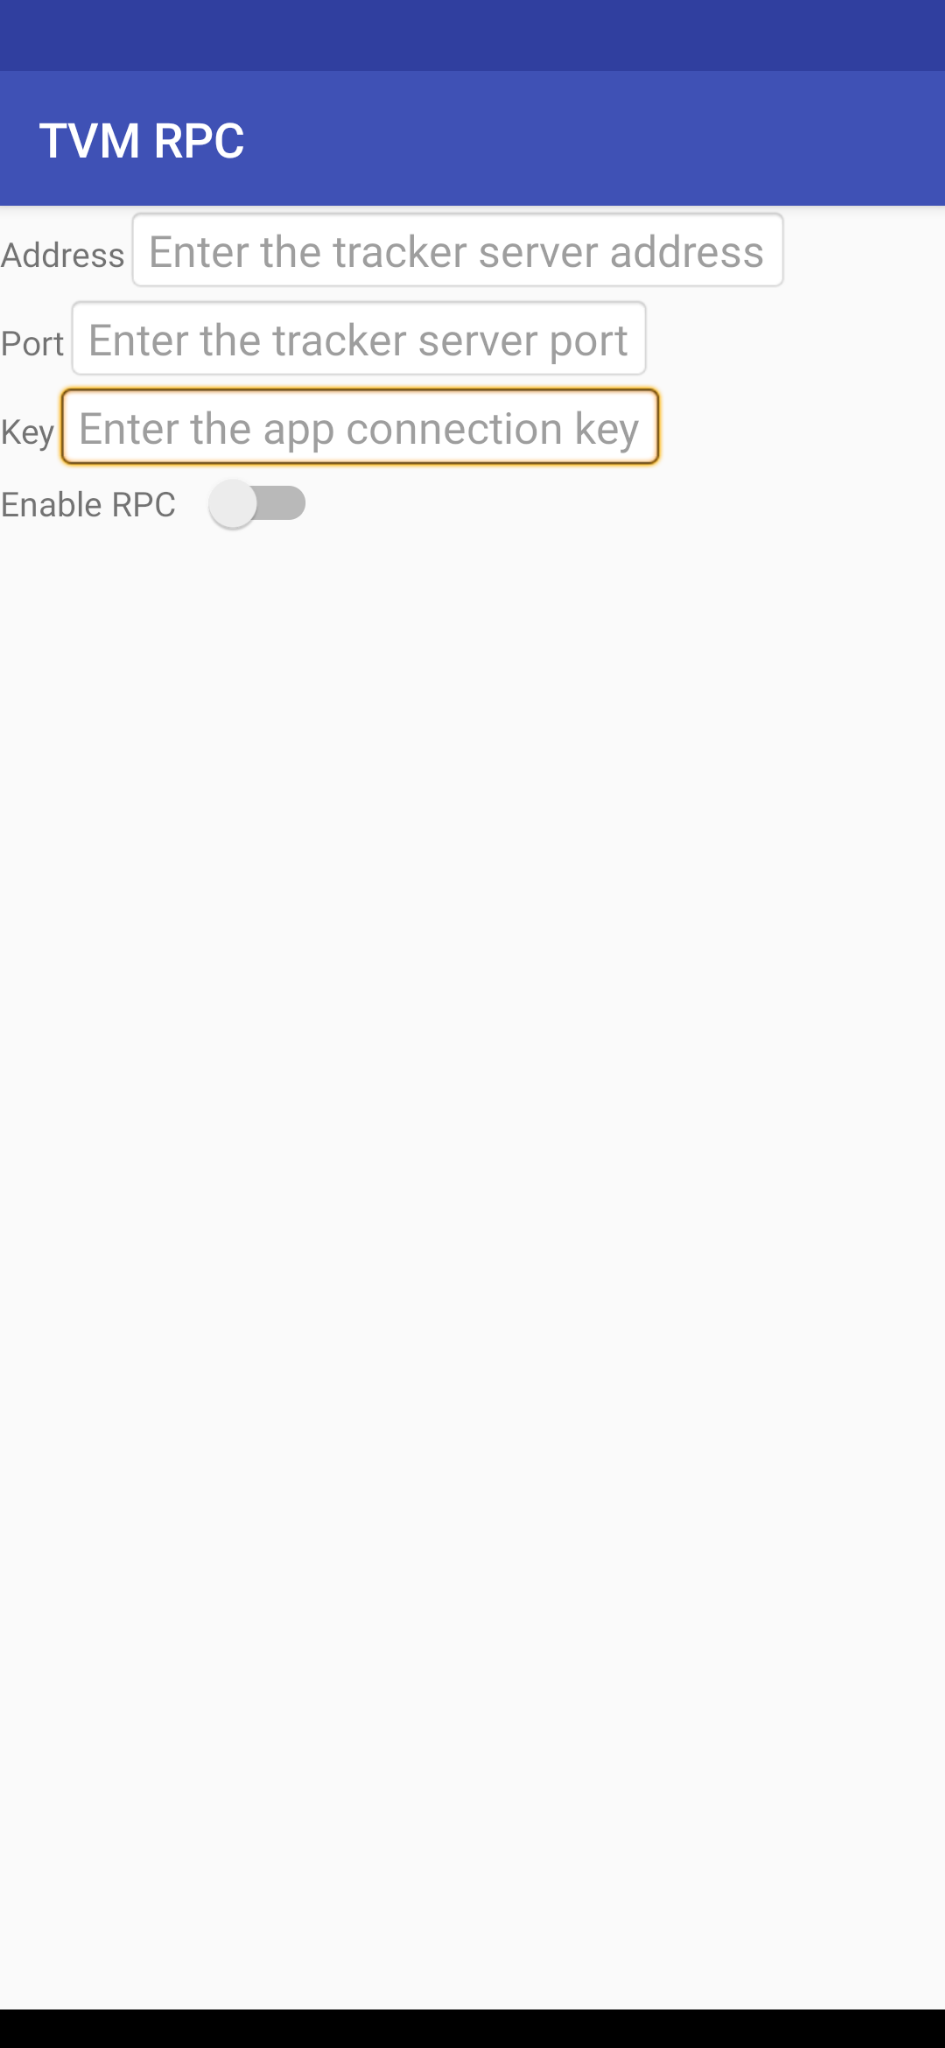
\includegraphics[width=180.bp]{figure/android_app.png}
    \caption{Android Rpc App界面}
    \label{android_rpc_app}
\end{figure}


\subsection{构建VTA模拟器}
该部分介绍VTA模拟器的编译环境,编译步骤以及VTA的配置参数。

\subsubsection{编译环境}

VTA模拟器的编译环境,采用64位Ubuntu系统,intel i5 10210U CPU,Nidia MX250 GPU。依赖的Cuda版本为11.1,Cudnn版本为8.0.5,LLVM版本为10。编译工具GCC版本为9.3.0,CMake版本为3.16.3,Make版本为4.2.0。

\subsubsection{编译流程}

首先,需要编译TVM的动态链接库,同时需要按照如下代码\ref{vta_environment}设置环境变量:

\begin{lstlisting}[
    language={bash},
    caption={VTA环境变量},
    label={vta_environment}
]
export TVM_PATH=/path/to/TVM
export VTA_HW_PATH=/path/to/TVM/3rdparty/vta-hw
\end{lstlisting}

其次,需要编译VTA的动态链接库,按照如下代码\ref{vta_compile}来进行动态链接库的编译:

\begin{lstlisting}[
    language={},
    caption={VTA编译流程},
    label={vta_compile}
]
cd <tvm-root>
mkdir build
cp cmake/config.cmake build/.
echo 'set(USE_VTA_FSIM ON)' >> build/config.cmake
cd build
cmake ..
make -j4
\end{lstlisting}

最后,通过修改PYTHONPATH环境变量,将VTA的Python前端代码加入到Python的包查找路径中,来进行使用。

\subsubsection{VTA参数}

VTA作为一个可自定义的深度学习加速器,可以通过修改一些配置参数来改变硬件的配置。本论文中用到的参数如下,其中具体的值为取对数后的值:
\begin{itemize}
    \item {TARGET:VTA部署的硬件设备,可以是sim(模拟器)或FPGA。本论文中使用sim。}
    \item {LOG\_INP\_WIDTH:输入向量的宽度。本论文中使用3。}
    \item {LOG\_WGT\_WIDTH:权重向量的宽度。本论文中使用3。}
    \item {LOG\_ACC\_WIDTH:累加器的数据宽度。本论文中使用5。}
    \item {LOG\_BATCH:VTA矩阵乘法元语中输入输出向量的维度0。本论文中使用0。}
    \item {LOG\_BLOCK:VTA矩阵乘法元语中输入输出向量的维度1。本论文中使用4。}
    \item {LOG\_UOP\_BUFF\_SIZE:微指令缓存的大小以比特为单位。本论文中使用15。}
    \item {LOG\_INP\_BUFF\_SIZE:输入向量缓存的大小以比特为单位。本论文中使用15。}
    \item {LOG\_WGT\_BUFF\_SIZE:权重向量缓存的大小以比特为单位。本论文中使用18。}
    \item {LOG\_ACC\_BUFF\_SIZE:累加器缓存的大小以比特为单位。本论文中使用17。}
\end{itemize}


\section{平台实现}

该部分具体介绍异构计算平台的各个模块以及模块的实现细节。

\subsection{编译模块}

使用TVM对多种框架的模型进行编译,同时使用具体的框架的接口来进行模型文件的加载,得到模型的对象后使用TVM的接口对模型对象进行编译得到中间表示的计算图和模型的参数。

本平台分别对支持的每种深度学习框架实现一个编译其模型的函数,本平台支持的编译函数如下:
\begin{itemize}
    \item {compile\_pytorch}
    \item {compile\_tensorflow}
    \item {compile\_keras}
    \item {compile\_onnx}
\end{itemize}

这些函数的参数都相同,如下所示:
\begin{itemize}
    \item {model:用户待编译的模型对象。}
    \item {input\_shape:模型输入向量的形状。}
    \item {kwargs:用户输入的其他参数。}
\end{itemize}

下面以compile\_pytorch函数为例,展示函数内部的编译的具体细节。

\begin{lstlisting}[
    language={python},
    caption={compile\_pytorch函数},
    label={compile_pytorch}
]
def compile_pytorch(model: torch.nn.Module, input_shape: list, kwargs):
    input_name = 'input0'
    input_data = torch.randn(input_shape)
    
    model.eval()
    # 调用Pytorch的接口,把模型转换为Torch Script格式
    scripted_model = torch.jit.trace(model, input_data).eval()

    shape_list = [(input_name, input_shape)]

    # 调用TVM的编译API进行模型的编译
    mod, params = relay.frontend.from_pytorch(scripted_model, input_infos=shape_list, **kwargs)

    return mod, params
\end{lstlisting}


\subsection{部署模块}

该部分分别介绍部署到本地,安卓设备,树莓派和VTA的具体实现细节。


\subsubsection{部署到本地}

TVM把得到的计算图的中间表示和参数部署到本地需要指定部署的target\_host和target,target\_host用来指定在CPU端执行的代码,一般为llvm,target用来指定具体的计算平台,在本地可以使用CPU计算或者GPU计算,所以target可以为llvm或cuda。下面为具体的代码\ref{deploy_local}:

\begin{lstlisting}[
    language={python},
    caption={部署到本地},
    label={deploy_local}
]
# 使用CPU进行计算
target = 'llvm'
target_host = 'llvm'
ctx = tvm.cpu(0)

# 得到动态链接库
with tvm.transform.PassContext(opt_level=3):
lib = relay.build(mod, target=target, target_host=target_host, params=params)
# 通过TVM执行动态链接库
m = graph_runtime.GraphModule(lib['default'](ctx))
m.set_input(input_name, input)
m.run()
tvm_output = m.get_output(0)
\end{lstlisting}


\subsubsection{部署到安卓设备}

部署到安卓与部署到本地不同,部署到安卓,需要让本地电脑能够与安卓设备进行通信,能够把得到的动态链接库上传到安卓设备,让动态链接库在安卓设备上执行。采用Rpc来使本地电脑和安卓进行通信,首先在本地,使用命令python -m tvm.exec.rpc\_tracker --host=<host> --port=<port>来创建一个Rpc的服务端。在安卓设备上,使用前文构建安装的App,输入指定的ip和端口,这样就可以使安卓设备和本地进行通信。使用TVM部署到安卓,同样需要指定target\_host和target,target\_host是在安卓端的CPU执行的代码,通常为llvm,target是安卓端的计算平台,可以是CPU,OpenCL和Vlukan。其次,在创建可以在安卓端执行的动态链接库时,因为安卓端的架构和本地不同,所以不能使用本地的编译器,需要使用TVM的ndk工具进行编译,然后将此上传到安卓端,下面是具体的代码\ref{deploy_android}:

\begin{lstlisting}[
    language={python},
    caption={部署到安卓},
    label={deploy_android}
]
with tvm.transform.PassContext(opt_level=3):
lib = relay.build(mod, target=target, params=params)

# 使用ndk来编译为动态链接库
fcompile = ndk.create_shared
lib.export_library('models/net.so', fcompile)

# 创建一个Rpc tracker来进行通信
tracker_host = os.environ.get('TVM_TRACKER_HOST', '0.0.0.0')
tracker_port = int(os.environ.get('TVM_TRACKER_PORT', '9190'))
key = 'android'
tracker = rpc.connect_tracker(tracker_host, tracker_port)
remote = tracker.request(key, priority=0, session_timeout=60)

# 上传动态链接库到Android端
remote.upload('models/net.so')
rlib = remote.load_module('net.so')

# 指定使用OpenCL进行计算
dev = remote.cl(0)
module = runtime.GraphModule(rlib['default'](dev))
module.set_input(input_name, tvm.nd.array(x.astype(dtype)))
module.run()
out = module.get_output(0)
\end{lstlisting}

\subsubsection{部署到树莓派}

树莓派是基于Linux的单片机,处理器采用ARM架构。与部署在安卓设备相同,同样需要使用RPC与树莓派设备进行通信,在本地使用TVM编译出可执行代码后,使用RPC把可执行代码上传到树莓派设备,然后在树莓派设备上进行运行,具体的代码如下\ref{deploy_rasp}:

\begin{lstlisting}[
    language={python},
    caption={部署到树莓派},
    label={deploy_rasp}
]
with tvm.transform.PassContext(opt_level=3):
    lib = relay.build(func, tvm.target.arm_cpu('rasp3b), params=params)

remote = rpc.conncet(host, port)
lib_fname = lib.export_library('net.tar')
remote.upload(lib_fname)
rlib = remote.load_module('net.tar')

dev = remote.cpu(0)
module = runtime.GraphModule(rlib["default"](dev))

module.set_input("data", tvm.nd.array(x.astype("float32")))
module.run()
out = module.get_output(0)
top1 = np.argmax(out.asnumpy())
print("TVM prediction top-1: {}".format(synset[top1]))
\end{lstlisting}

\subsubsection{部署到VTA}

通过TVM编译处VTA指令集的可执行代码,得到可执行代码后,在本地的VTA模拟器执行该代码。与部署到其他设备不同的是,VTA的选项中,只支持输入和权重的向量为8位,所以在生成代码之前还需要对模型进行量化,具体的代码如下\ref{deploy_vta}:

\begin{lstlisting}[
    language={python},
    caption={部署到VTA},
    label={deploy_vta}
]
remote = rpc.LocalSession()
with tvm.transform.PassContext(opt_level=3):
    with relay.quantize.qconfig(global_scale=8.0, skip_conv_layers=[0]):
        mod = relay.quantize.quantize(mod, params=params)
    relay_prog = graph_pack(
        mod["main"],
        env.BATCH,
        env.BLOCK_OUT,
        env.WGT_WIDTH,
        start_name=pack_dict[model][0],
        stop_name=pack_dict[model][1],
        device_annot=(env.TARGET == "sim"),
    )
with vta.build_config(opt_level=3, disabled_pass={"AlterOpLayout"}):
    graph, lib, params = relay.build(
        relay_prog, target=target, params=params, target_host=env.target_host
    )
\end{lstlisting}


\section{接口实现}

对于平台的接口实现来说,通过一个基类BaseTVMHelper来表示共通的编译部署流程,对于每种具体的设备,通过继承该基类来实现一个针对具体设备的编译部署流程,对于本平台支持的4种设备,共实现如下4哥类:
\begin{itemize}
    \item {LocalTVMHelper}
    \item {AndroidTVMHelper}
    \item {RaspTVMHelper}
    \item {VtaTVMHelper}
\end{itemize}

\begin{table}
    \centering
    \caption{接口基本参数}
    \label{interface_base_params}
    \begin{tabular}{c|c|c}
        \hline
        变量                      & 类型     & 含义        \\ \hline
        device                  & string & 部署到的设备    \\ \hline
        frame                   & string & 模型使用的框架   \\ \hline
        model                   & object & 模型对象      \\ \hline
        input\_shape            & list   & 模型输入的形状   \\ \hline
        opt\_level              & int    & 优化等级      \\ \hline
        target                  & string & 设备上的计算平台  \\ \hline
        compile\_arg\_dict=\{\} & dict   & 额外的模型编译参数 \\ \hline
    \end{tabular}
\end{table}

上表\ref{interface_base_params}是接口的基本参数,其中,device是部署到的设备,目前支持local,android,rasp,和vta。frame是模型的框架,目前支持pytorch,tensorflow,keras,和onnx。model是具体框架加载后的模型对象。input\_shape是模型输入的形状。opt\_level是模型优化的等级,目前支持1,2,3。target是具体设备上的计算平台,部署到不同设备上target的值不同,如部署到local,target为cpu或cuda。部署到android设备上,target为cpu,opencl,或vulkan。

部署到本地的接口和部署到VTA的接口参数与基本参数相同,部署到安卓设备和树莓派设备上还需要一些额外的参数,如下表\ref{interface_extra_params}所示。

\begin{table}
    \centering
    \caption{接口额外参数}
    \label{interface_extra_params}
    \begin{tabular}{c|c|c}
        \hline
        变量            & 类型     & 含义                 \\ \hline
        tracker\_host & string & 创建Rpc Tracker的host \\ \hline
        tracker\_port & int    & 创建Rpc Tracker的端口   \\ \hline
        key           & string & 连接Rpc的key          \\ \hline
    \end{tabular}
\end{table}

下面通过调用本接口来把Pytorch模型部署到本地来展示接口的具体使用:

\begin{lstlisting}[
    language={python},
    caption={本地接口使用},
    label={use_interface_local}
]
import torch
import torchvision
import numpy as np
# 引入Helper类
from PlatfromTVM import LocalTVMHelper

# 获得模型
model = getattr(torchvision.models, ‘resnet18’)(pretrained=True)

# 部署到local设备,使用CPU计算
deployed_model = LocalTVMHelper(device=’local’,frame=’pytorch’
   model=model,input_shape=[1,3,224,224],opt_level=3,target=’cpu’)
# 通过部署的模型计算
out = deployed_model(input)
\end{lstlisting}

下图\ref{compare}是使用该平台和不是该平台把模型部署到安卓设备上的代码对比,左侧是使用该平台,右侧是不使用该平台:

\begin{figure}[h!]
    \centering
    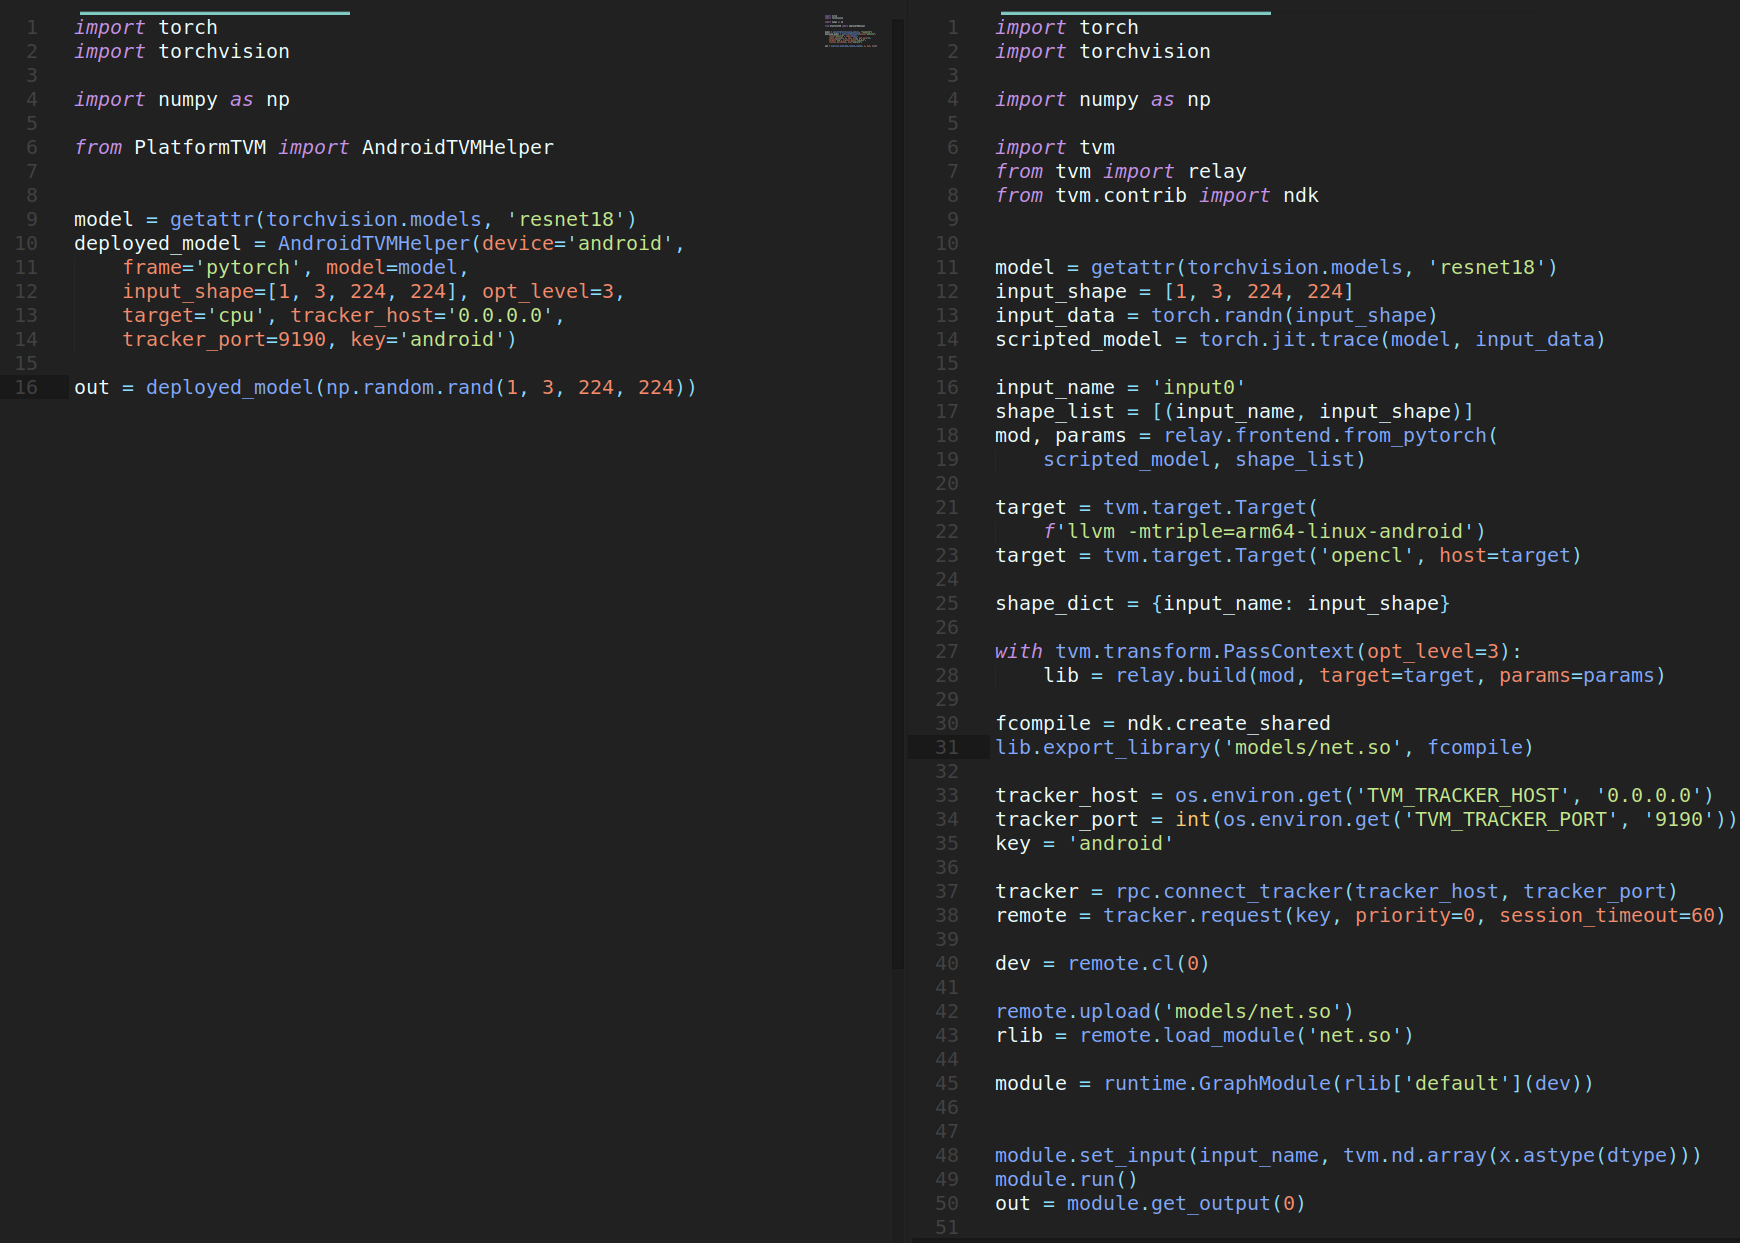
\includegraphics[]{figure/compare.png}
    \caption{代码对比}
    \label{compare}
\end{figure}

可以看到,使用该平台大大简化了模型编译部署的难度,同时使用户不需要了解使用TVM编译部署的具体细节以及是使用Rpc通信的具体细节。